% Lab 01: Python Dictionary - Storing Disease Information
% LaTeX Beamer Presentation

\documentclass[aspectratio=169]{beamer}

% Theme and colors
\usetheme{Madrid}
\usecolortheme{whale}
\setbeamertemplate{navigation symbols}{}
\setbeamertemplate{footline}[frame number]

% Packages
\usepackage{listings}
\usepackage{graphicx}
\usepackage{tikz}
\usepackage{fontspec}

% Code styling
\lstset{
    language=Python,
    basicstyle=\ttfamily\small,
    keywordstyle=\color{blue}\bfseries,
    stringstyle=\color{red},
    commentstyle=\color{green!60!black},
    showstringspaces=false,
    frame=single,
    backgroundcolor=\color{gray!10},
    breaklines=true
}

% Title information
\title{Lab 01: Python Dictionary}
\subtitle{Storing Disease Information for RAG Systems}
\author{CSI403 - Full Stack Program Development}
\date{}

\begin{document}

% ============================================
% TITLE SLIDE
% ============================================
\begin{frame}
    \titlepage
\end{frame}

% ============================================
% AGENDA
% ============================================
\begin{frame}{Today's Agenda}
    \begin{columns}
        \begin{column}{0.5\textwidth}
            \textbf{Learning:}
            \begin{itemize}
                \item What is a Dictionary?
                \item Why use Dictionary in RAG?
                \item Creating Dictionaries
                \item Accessing \& Modifying Data
                \item List of Dictionaries
            \end{itemize}
        \end{column}
        \begin{column}{0.5\textwidth}
            \textbf{Time:}
            \begin{itemize}
                \item Lecture: 30 min
                \item Tutorial: 60 min
                \item Break: 15 min
                \item Exercise: 45 min
                \item Submit: 15 min
                \item Q\&A: 15 min
            \end{itemize}
        \end{column}
    \end{columns}
\end{frame}

% ============================================
% WHAT IS A DICTIONARY?
% ============================================
\begin{frame}{What is a Dictionary?}
    \begin{center}
        \textbf{A Dictionary stores data as KEY-VALUE pairs}
    \end{center}
    
    \vspace{0.5cm}
    
    \begin{columns}
        \begin{column}{0.45\textwidth}
            \textbf{Real Dictionary:}
            \begin{itemize}
                \item Word $\rightarrow$ Definition
                \item ``Apple'' $\rightarrow$ ``A fruit''
                \item ``Python'' $\rightarrow$ ``A programming language''
            \end{itemize}
        \end{column}
        \begin{column}{0.45\textwidth}
            \textbf{Python Dictionary:}
            \begin{itemize}
                \item Key $\rightarrow$ Value
                \item ``name'' $\rightarrow$ ``Rubella''
                \item ``symptoms'' $\rightarrow$ ``fever, rash''
            \end{itemize}
        \end{column}
    \end{columns}
    
    \vspace{0.5cm}
    
    \begin{block}{Key Point}
        Use \textbf{keys} to quickly find \textbf{values} - like looking up a word!
    \end{block}
\end{frame}

% ============================================
% DICTIONARY VISUALIZATION
% ============================================
\begin{frame}{Dictionary Visualization}
    \begin{center}
        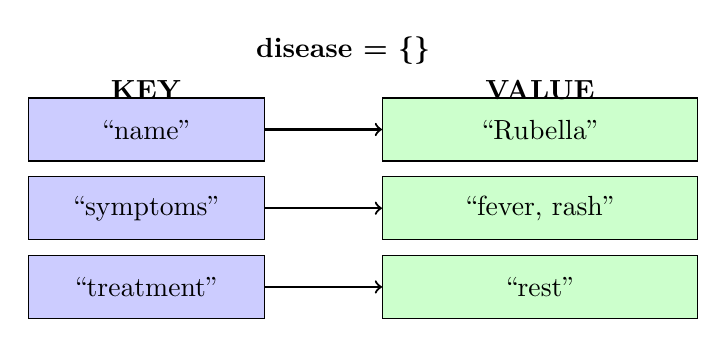
\begin{tikzpicture}[
            box/.style={rectangle, draw, minimum width=3cm, minimum height=0.8cm, fill=blue!20},
            value/.style={rectangle, draw, minimum width=4cm, minimum height=0.8cm, fill=green!20},
            arrow/.style={->, thick}
        ]
            % Title
            \node at (2.5, 3) {\textbf{disease = \{\}}};
            
            % Keys
            \node[box] (k1) at (0, 2) {``name''};
            \node[box] (k2) at (0, 1) {``symptoms''};
            \node[box] (k3) at (0, 0) {``treatment''};
            
            % Values
            \node[value] (v1) at (5, 2) {``Rubella''};
            \node[value] (v2) at (5, 1) {``fever, rash''};
            \node[value] (v3) at (5, 0) {``rest''};
            
            % Arrows
            \draw[arrow] (k1) -- (v1);
            \draw[arrow] (k2) -- (v2);
            \draw[arrow] (k3) -- (v3);
            
            % Labels
            \node at (0, 2.5) {\textbf{KEY}};
            \node at (5, 2.5) {\textbf{VALUE}};
        \end{tikzpicture}
    \end{center}
\end{frame}

% ============================================
% WHY DICTIONARY IN RAG?
% ============================================
\begin{frame}[fragile]{Why Use Dictionary in RAG Systems?}
    \begin{center}
        \textbf{RAG = Retrieval-Augmented Generation}
    \end{center}
    
    \vspace{0.3cm}
    
    In RAG systems, we need to store \textbf{documents} with \textbf{metadata}:
    
    \begin{columns}
        \begin{column}{0.5\textwidth}
\begin{lstlisting}
document = {
    "title": "Rubella",
    "content": "Rubella is...",
    "source": "medthai.com",
    "date": "2024-01-15"
}
\end{lstlisting}
        \end{column}
        \begin{column}{0.45\textwidth}
            \textbf{Benefits:}
            \begin{itemize}
                \item Organized structure
                \item Fast key lookup
                \item Easy to extend
                \item JSON compatible
            \end{itemize}
        \end{column}
    \end{columns}
    
    \vspace{0.3cm}
    
    \begin{alertblock}{Important}
        Almost all RAG systems use dictionaries to store documents!
    \end{alertblock}
\end{frame}

% ============================================
% CREATING A DICTIONARY
% ============================================
\begin{frame}[fragile]{Creating a Dictionary}
    \textbf{Method 1: Empty dictionary, then add}
\begin{lstlisting}
# Create empty dictionary
disease = {}

# Add key-value pairs
disease["name"] = "Rubella"
disease["symptoms"] = "fever, rash"
\end{lstlisting}
    
    \vspace{0.3cm}
    
    \textbf{Method 2: Create with data}
\begin{lstlisting}
# Create with initial data
disease = {
    "name": "Rubella",
    "symptoms": "fever, rash",
    "treatment": "rest"
}
\end{lstlisting}
\end{frame}

% ============================================
% ACCESSING VALUES
% ============================================
\begin{frame}[fragile]{Accessing Dictionary Values}
    \textbf{Using square brackets [ ]}
\begin{lstlisting}
disease = {
    "name": "Rubella",
    "symptoms": "fever, rash"
}

# Access by key
print(disease["name"])       # Output: Rubella
print(disease["symptoms"])   # Output: fever, rash
\end{lstlisting}
    
    \vspace{0.3cm}
    
    \textbf{Using .get() method (safer)}
\begin{lstlisting}
# Returns None if key doesn't exist
print(disease.get("treatment"))        # Output: None
print(disease.get("treatment", "N/A")) # Output: N/A
\end{lstlisting}
\end{frame}

% ============================================
% MODIFYING DICTIONARY
% ============================================
\begin{frame}[fragile]{Adding \& Modifying Values}
\begin{lstlisting}
disease = {"name": "Rubella", "symptoms": "fever"}

# ADD a new key
disease["treatment"] = "rest"
disease["prevention"] = "vaccination"

# MODIFY existing value
disease["symptoms"] = "fever, rash, fatigue"

# DELETE a key
del disease["prevention"]

print(disease)
# {'name': 'Rubella', 'symptoms': 'fever, rash, 
#  fatigue', 'treatment': 'rest'}
\end{lstlisting}
\end{frame}

% ============================================
% LIST OF DICTIONARIES
% ============================================
\begin{frame}[fragile]{List of Dictionaries}
    \textbf{Store multiple items using a list:}
\begin{lstlisting}
diseases = [
    {"name": "Rubella", "symptoms": "fever, rash"},
    {"name": "Cholera", "symptoms": "diarrhea"},
    {"name": "GERD", "symptoms": "heartburn"}
]

# Access first disease
print(diseases[0]["name"])  # Output: Rubella

# Access second disease symptoms
print(diseases[1]["symptoms"])  # Output: diarrhea
\end{lstlisting}
    
    \begin{block}{This is how RAG systems store documents!}
        Each document = 1 dictionary in a list
    \end{block}
\end{frame}

% ============================================
% LOOPING THROUGH DICTIONARIES
% ============================================
\begin{frame}[fragile]{Looping Through Data}
    \textbf{Loop through list of dictionaries:}
\begin{lstlisting}
diseases = [
    {"name": "Rubella", "symptoms": "fever, rash"},
    {"name": "Cholera", "symptoms": "diarrhea"},
    {"name": "GERD", "symptoms": "heartburn"}
]

# Display all disease names
for disease in diseases:
    print(disease["name"])

# Output:
# Rubella
# Cholera
# GERD
\end{lstlisting}
\end{frame}

% ============================================
% USEFUL DICTIONARY METHODS
% ============================================
\begin{frame}[fragile]{Useful Dictionary Methods}
\begin{lstlisting}
disease = {"name": "Rubella", "symptoms": "fever"}

# Get all keys
print(disease.keys())   # dict_keys(['name', 'symptoms'])

# Get all values
print(disease.values()) # dict_values(['Rubella', 'fever'])

# Get all key-value pairs
print(disease.items())  # dict_items([...])

# Check if key exists
print("name" in disease)       # True
print("treatment" in disease)  # False
\end{lstlisting}
\end{frame}

% ============================================
% SUMMARY
% ============================================
\begin{frame}{Summary}
    \begin{columns}
        \begin{column}{0.5\textwidth}
            \textbf{What we learned:}
            \begin{itemize}
                \item Dictionary = key-value pairs
                \item Create: \texttt{\{\}} or \texttt{dict()}
                \item Access: \texttt{d[``key'']} or \texttt{d.get(``key'')}
                \item Add/Modify: \texttt{d[``key''] = value}
                \item Delete: \texttt{del d[``key'']}
                \item List of dicts for multiple items
            \end{itemize}
        \end{column}
        \begin{column}{0.45\textwidth}
            \textbf{Next steps:}
            \begin{enumerate}
                \item Complete Tutorial Notebook
                \item Do 5 Exercises
                \item Push to GitHub
                \item Check auto-grading score
            \end{enumerate}
        \end{column}
    \end{columns}
    
    \vspace{0.5cm}
    
    \begin{block}{Remember}
        Dictionaries are the foundation of storing documents in RAG systems!
    \end{block}
\end{frame}

% ============================================
% EXERCISES PREVIEW
% ============================================
\begin{frame}{Exercise Preview (5 exercises, 100 points)}
    \begin{enumerate}
        \item \textbf{Create a dictionary} (20 pts) \\
              Create a dictionary for ``Dengue Fever'' disease
        \item \textbf{Add a new key} (20 pts) \\
              Add ``prevention'' key to your dictionary
        \item \textbf{Access values} (20 pts) \\
              Print the symptoms of the disease
        \item \textbf{Create list of dictionaries} (20 pts) \\
              Create a list containing 3 diseases
        \item \textbf{Loop through data} (20 pts) \\
              Loop and print all disease names
    \end{enumerate}
    
    \vspace{0.3cm}
    
    \begin{alertblock}{Time: 45 minutes}
        Work on \texttt{exercise/Lab01\_Exercise.ipynb}
    \end{alertblock}
\end{frame}

% ============================================
% QUESTIONS
% ============================================
\begin{frame}
    \begin{center}
        \Huge \textbf{Questions?}
        
        \vspace{1cm}
        
        \Large Let's start the Tutorial!
        
        \vspace{0.5cm}
        
        \normalsize Open: \texttt{tutorial/Lab01\_Tutorial.ipynb}
    \end{center}
\end{frame}

\end{document}
